\documentclass{article}

% Required packages
\usepackage{graphicx}
\usepackage{array}
\usepackage{geometry}
\usepackage{caption}
\usepackage{amsmath,amssymb}  % Added for mathematical symbols
\usepackage{url}  % For URLs in bibliography

% Set page margins
\geometry{margin=1in}

% Title and author information
\title{\Large\textbf{Code Companion: Using ML to Detect Vulnerabilities in Code}}
\date{}  % Remove date

\begin{document}

% Title page
\begin{titlepage}
\begin{center}
\vspace*{2cm}
{\huge\textbf{Code Companion: Using ML to Detect Vulnerabilities in Code}\par}
\vspace{2cm}

% Authors table
\begin{tabular*}{\textwidth}{@{\extracolsep{\fill}} *{4}{c}}
    \textbf{Andrew Bevington} & \textbf{Sara Madani} & \textbf{Bryan O'Keefe} & \textbf{Alex Velsmid} \\[0.0cm]
    Computer Science & Math & Computer Science & Computer Science \\[0.0cm]
    Boston College & Bocconi University & Boston College & Boston College \\[0.0cm]
    Class of 2025 & Class of 2025 & Class of 2026 & Class of 2026 \\
\end{tabular*}

\vfill
\today
\end{center}
\end{titlepage}

%% Start two-column format from here
% \twocolumn

\section*{Abstract}
A big problem for every software engineer and tech company is ensuring their applications are
secure. Without proper security, vulnerabilities in code can allow for hackers to gain
unauthorized access to user data and private source code. Exploits in code can negatively
affect consumers and products, which is a big problem for companies. In the past, thousands
of lines of code would have to be manually reviewed by professionals to find and remove these
vulnerabilities. The goal of this project is to create a machine learning algorithm that
automates this process by taking in a function written in C and running a binary classification
model on the function to label it as vulnerable or non-vulnerable. This would alleviate the pain
of manual review, and help programmers create more secure programs.

\section{Introduction}
With the rapidly increasing pace of software development as a result of modern tools like generative AI,
the need to ensure code security is becoming increasingly more valuable. According to IBM's Cost of a
Data Breach Report 2024, the average global cost of a data breach is \$4.88 million, a 10\% increase from
2023. This highlights the critical importance of cybersecurity as more and more aspects of modern life become
digitized and connected. Therefore, cybersecurity is important in modern society as unauthorized access to
private records and data can have severe effects. In an effort to increase cybersecurity and code review
efficiency, our goal is to create a machine learning model to accurately detect flaws in code. In order to
do so, the model would take code files as input and output areas and behaviors that are vulnerable, their
severity, and suggestions to improve. Currently, there are multiple issues present with adapting a machine
learning model to cyber security efforts. These issues are noted in \cite{Arp2024}, that discusses how many top-tier security papers
from the past decade that rely on machine learning concepts exhibit three main common issues. These problems include inappropriate threat
models — where the assumed threats are not reflective of actual security risks – adversarial vulnerabilities
– where malicious inputs can deceive machine learning models – and sampling bias – when training data does
not accurately represent real-world data. In model training, the third issue of sampling bias greatly impacted the performance
of the model in a negative way if ignored and positively if considered and fixes. Before developing a model, data will be taken 
from multiple databases in order to obtain training data which is formatted and filtered to avoid duplications and inconsistencies
in syntax and layout. After collecting the data we aim to traverse through multiple experiments. Starting with the OpenAI API as
a baseline we diversify to a GNN as well as a basic linear model used to create an Adaboost style gradient boosting network.


\subsection{Data}
There are two sources of data which we have explored. The first of these is the 
DiverseVul dataset \cite{chen2023diversevulnewvulnerablesource}, which has been cited and used in over a hundred research papers. This dataset contains a large number of vulnerabilities written in C/C++.
These have been split into two categories: those which contain vulnerabilities and those
where vulnerabilities are not present determined by the "target" entry of the json. In the vulnerabilities present category, there are 
18,945 files, and in the vulnerabilities not present category, there are 330,492 
examples of code. When in its raw form each of these entries contains information such as the function itself, the github commit it came from,
the target (0 - non vulnerable, 1 - vulnerable), the CVSS score and other metada relating to the git commit that it originally came from. However, we saw 
most of this information as unnecessary so we programatically pruned the dataset to contain only the function itself alongside the "target" of 1 or 0. This
was mainly to shrink the overall size of the database file as well as guarantee that the model learns from only the function and not any other 
proprietary information. 

Another dataset that we have explored is the PrimeVul \cite{ding2024vulnerabilitydetectioncodelanguage} dataset. This dataset is an improvement on the DiverseVul dataset in that it was created with more attention and human
intervention. The dataset contains 6,968 vulnerable functions as well as 228,000 non-vulnerable functions. The data is also pre-split into training and testing sets. This ensures
that there is no code duplication between the two sets. The PrimeVul dataset is the one that
we will start our experimentation with and will serve as the main dataset for our project.
If we find that we need more data, then we will migrate to the DiverseVul dataset. However,
if this is deemed necessary, then we will need to take steps to ensure that the data is clean.
This will likely involve removing duplicates and ensuring that the data is correctly labeled,
all of which is possible with python scripts to reformat and refactor the data. 


\begin{figure}
\begin{verbatim}
{
  "idx": 0,
  "project": "openssl",
  "commit_id": "ca989269a2876bae79393bd54c3e72d49975fc75",
  "project_url": "https://github.com/openssl/openssl",
  "commit_url": "https://git.openssl.org/gitweb/?p=openssl.git;a=commit;h=ca989269a2876bae79393bd54c3e72d49975fc75",
  "commit_message": "Use version in SSL_METHOD not SSL structure [...]",
  "target": 1f
  "func": "long ssl_get_algorithm2(SSL *s)\n{\n [...] \n}",
  "func_hash": 255087747659226932756944884868284698117,
  "file_name": "None",
  "file_hash": null,
  "cwe": ["CWE-310"],
  "cve": "CVE-2013-6449",
  "cve_desc": "The ssl_get_algorithm2 function in ssl/s3_lib.c in OpenSSL before 1.0.2 obtains a certain version number from an incorrect data structure, which allows remote attackers to cause a denial of service (daemon crash) via crafted traffic from a TLS 1.2 client.",
  "nvd_url": "https://nvd.nist.gov/vuln/detail/CVE-2013-6449"
}
\end{verbatim}
\caption{Example of an entry in the PrimeVul database for a vulnerability in the OpenSSL project (CVE-2013-6449).}
\label{fig:primevul_example}
\end{figure}

\subsection{Behaviors}
In the general use case of this model we see it as having a fairly streamlined approach to scanning through code. In the correct usage, a user would upload a set of files to the model. From these files the model would then look through and determine where there are code vulnerabilities and their severity. In the best case we see the model being able to point out the line or lines of code where there is a code insecurity. With this identification would also come an explanation of why the code poses a risk, what the scale of that risk is, and some ways in which the user can fix the issue. This will be given to the user in the form of a text file or a chatbot-based system depending on how our experimentation progresses. 
It is easy to foresee errors in this ideal flow of information. The most common error which we are most likely to see would be an absence of identification of code vulnerabilities. If we feed it in code with vulnerabilities and the model fails to see these vulnerabilities then the model is not doing what it is supposed to be doing and not functioning in an optimal way. 

With the usage of a datasource like PrimeVul or DiverseVul we are able to create a model which can identify individual lines of code as well as large sections of vulnerable code. With its training on entire Git commits it will be able to function in an environment which more closely resembles that which a user is likely to upload to the model. It will be able to parse through the code and identify behaviours which a line by line model would not be able to see. Also, with the addition of the NIST database we are able to web scrape the provided link in order to allow the model to return a human-readable response explaining what the vulnerability is, how it works in the code, and just how bad it could be if it is left to be unchecked. 

\section{Related Works}

Before delving into the works strictly related to our study, we researched some papers about the chosen topic in order to get a better understanding of past concerns and focuses. What we found is that actually it's been a deeply investigated topic, especially by US researchers, resulting in lots of pre-existing literature. Thanks to these we have an overview over how codes' vulnerabilities have been valued in the past, also related to their consequences and implications, which methods have been used to detect them and how effective the analysis was \cite{LIANG2025104098}. Also, some of the papers investigate further the possible future challenges and prospects in this field, highlighting the problems that we still encounter, despite the giant steps that have been taken, in finding realistic and at the same time accurate data and interpret perfectly the models, since many advanced algorithms make it difficult to understand why certain vulnerabilities are flagged \cite{harer2018automatedsoftwarevulnerabilitydetection}.

The main agents in the vulnerability workspace are large-scale models such as ChatGPT \cite{openai2024gpt4} which allows for general querying of code, as well as StarCoder2 \cite{lozhkov2024starcoder2stackv2}, a LLM trained on a large amount of data related to coding specifically. The prior benchmark for model success was running them on the BigVul dataset. However, upon further research, it was found that this dataset was flawed and a poor representation of real world applications. A large issue was in code duplications as well as poor labeling of data. When trained on PrimeVul, a more refined and accurate dataset, StarCoder2 went from a 68.7\% F1 score to a 3.03\% F1 score \cite{ding2024vulnerabilitydetectioncodelanguage}. It is found through experimentation that these large pre-trained models are ineffective at accurately finding and diagnosing malicious code in a real world environment and that novel approaches need to be made to allow for real world applications of this product. \cite{ding2024vulnerabilitydetectioncodelanguage}

Flawfinder is a naive approach to vulnerability detection. This application works by searching within a code file for known vulnerabilities, such as buffer overflows, format string problems, and more. This simple approach allows for quick identification of simple, surface-level bugs, however, cannot understand data types of function parameters, nor analyze control flow or data flow. To perform deeper analysis on vulnerabilities, machine learning techniques will be necessary.


AMPLE is the state-of-the-art vulnerability detection model that uses graph neural networks (GNNs). This model works by taking in input source code and converting it into a code property graph (CPG). Then, it uses type-based graph simplification and variable-based graph simplification to reduce size and complexity of the graph. Then, the code graphs are processed through an edge-aware graph convolutional network (GCN), which computes node vectors according to their type, and then enhances node representation based on a multi-head attention mechanism and returns an edge-enhanced node representation matrix. Then, a kernel-scaled representation module is used to analyze close and long range relationships between nodes. To do this, kernel-scaled convolutions are used on the edge-enhanced node representation matrix using a large and small kernel. Then, two fully-connected layers and a softmax function are used to perform binary classification. AMPLE demonstrates massive improvements on other models, achieving 92.71\% accuracy on the Reveal dataset. A traditional token-based model, SySeVR, only achieves 74.33\% accuracy. 

In an attempt to improve upon existing graph-based approaches to vulnerability detection, such as AMPLE3, researchers developed ANGEL\cite{wen2023vulnerabilitydetectiongraphsimplification}, a novel approach to vulnerability detection, combining a GNN and a graph transformer (GT). In this model, code files are converted to code property graphs using Joern\cite{6956589}. The GNN provides details about local features from adjacent neighbors of each node. The GT leverages a multi-head self-attention mechanism to extract global features from the entire graph. In combination, both global and local relationships are captured, allowing for better detection of vulnerabilities that result from long-range dependencies. In addition, the AMPLE model falls short when dealing with large code graphs. To address this issue, ANGEL uses an self-adaptive importance-based graph simplification module consisting of multiple pooling layers. The simplification process will terminate when the graph size is below a certain threshold. Using the Reveal database, ANGEL achieves an 87.45\% accuracy. In comparison, Flawfinder achieves a 79.89\% accuracy. Additionally, SySeVR, a popular token-based method, only achieves 77.47\% accuracy. Compared to the state-of-the-art graph based model, AMPLE, ANGEL is 4.66\% more accurate on the Reveal dataset. In this work, we aim to leverage techniques used by ANGEL and AMPLE to achieve accurate vulnerability detection and risk scoring.

\section{Experimentation}
In this section we will outline the experiments that we have run in data collection and model comparison
and explain our findings for each of these iterations. 

\subsection{Data Collection}
For the collection and formatting of data we looked to simplify the json that we would supply the model with. To do this, we decreased the parameters and also got the ground truth CVSS scores from the NVD website in order to be able to provide the model with a ground truth to run a loss against. 

\begin{figure}
\begin{verbatim}
{
  "idx": 0,
  "func": "long ssl_get_algorithm2(SSL *s)\n{\n [...] \n}",
  "cve_id": "CVE-2013-6449",
  "cvss_score": "4.3",
  "cvss_severity": "MEDIUM",
  "func_hash": 255087747659226932756944884868284698117
}
\end{verbatim}
\caption{Example of a refined dataset for model training}
\label{fig:refined_example}
\end{figure}

The NVD api has a rate limiter of 100 calls per 30 seconds, however, this seemed to be high based on how efficiently our API was running. In failing efforts to try and speed this process up we tried: parallel calling and batch calling. In principle, being able to parallelize the calling would allow for multiple data points to be collected at once, however, regardless of how little we parallelized it still hit the rate limiter which resulted in CVSS score field not being populated. A similar issue occurred with batch calling as ideally we would be able to call 100 API's every 30 seconds. More generally, the API rate limiter even gave issues for single stream slow API calling as it would often return errors such as Status Code 503 which signaled that the rate limit was preventing further progress. In an attempt to handle this we implemented 3 attempts to retrieve the data with exponential time back off. The idea was to allow the rate limit to reset and retrieve the data. This implementation worked but it was too slow to be a plausible solution.

\subsection{ChatGPT}
As a baseline we decided to explore ChatGPT 3.5. We approached this by first converting the data which we had
from the large PrimeVul database into a more refined and focused dataset with the information that we needed
and nothing more. For this, we had to implement a web scraper in order to pull the ground truth CVSS scores
from the NVD website for each of the entries. After this was complete, we created a script which would send a 
uniform query to the ChatGPT API and measure the MSE of the GPT-generated CVSS scores compared to the 
ground truth scores from our web scraper. We found that the model averaged out with a loss of 4.81. We found 
this to be a poor performance especially in functions with no vulnerabilities which it was supposed to 
label with a CVSS score. Overall, ChatGPT was overly cautious, often assigning a higher score than the 
vulnerability deserved.

\begin{figure}[htbp]
    \centering
    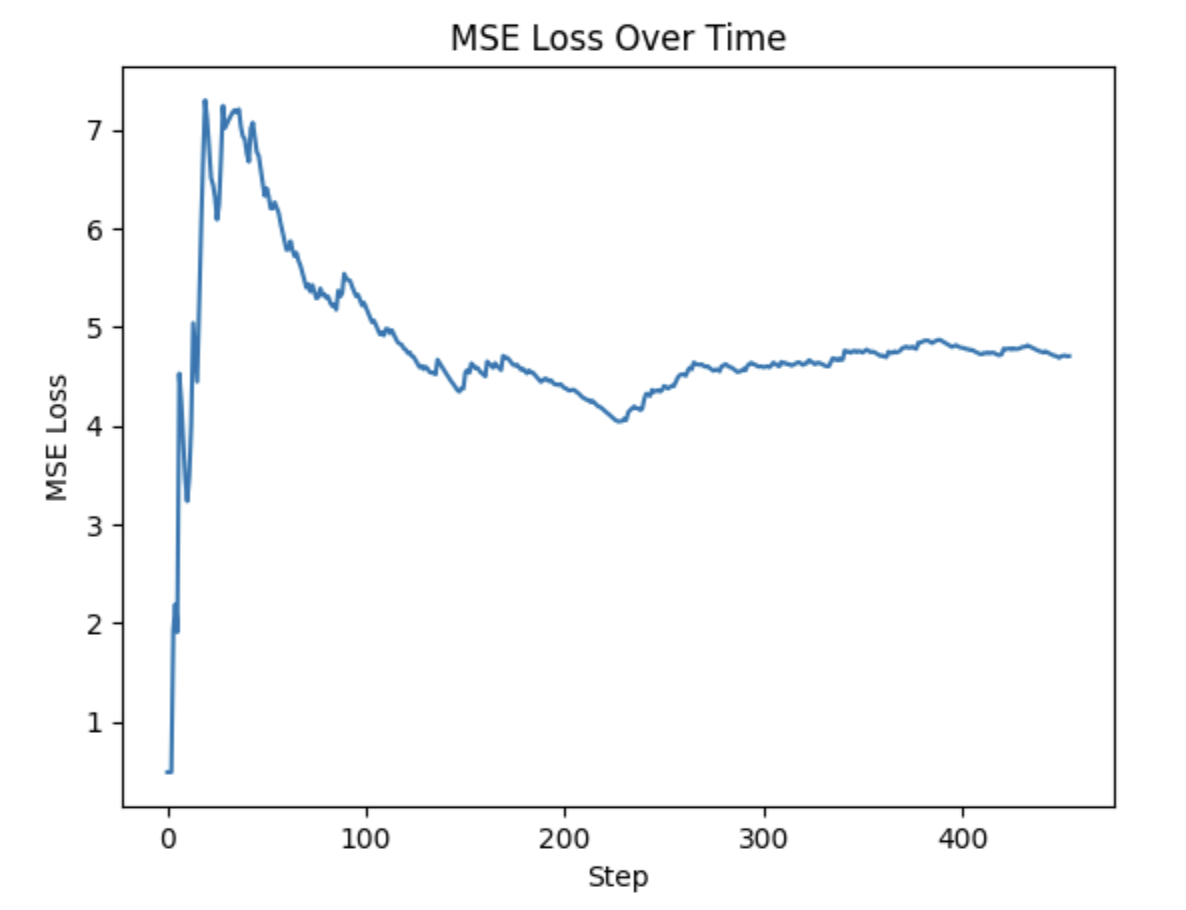
\includegraphics[width=0.6\textwidth]{images/gpt_loss.png}
    \caption{A graph of the MSE loss of ChatGPT 3.5}
    \label{fig:gpt_loss}
\end{figure}

As a follow up to this experiment, we implemented a naïve algorithm which "guesed" a constant risk score for
any function that it was given. For this, we iterated trough the risk scores from 0 - 10 and graphed the loss
for each to see which would be the most efficent and if any were more accurate than ChatGPT. We found that a 
guess of 3.2 was optimal for performance with a loss of 7.2. This was still worse than ChatGPT. WIth this we
were able to create the start of an algorithm and model hierarchy for performance on our data. 

\begin{figure}[htbp]
    \centering
    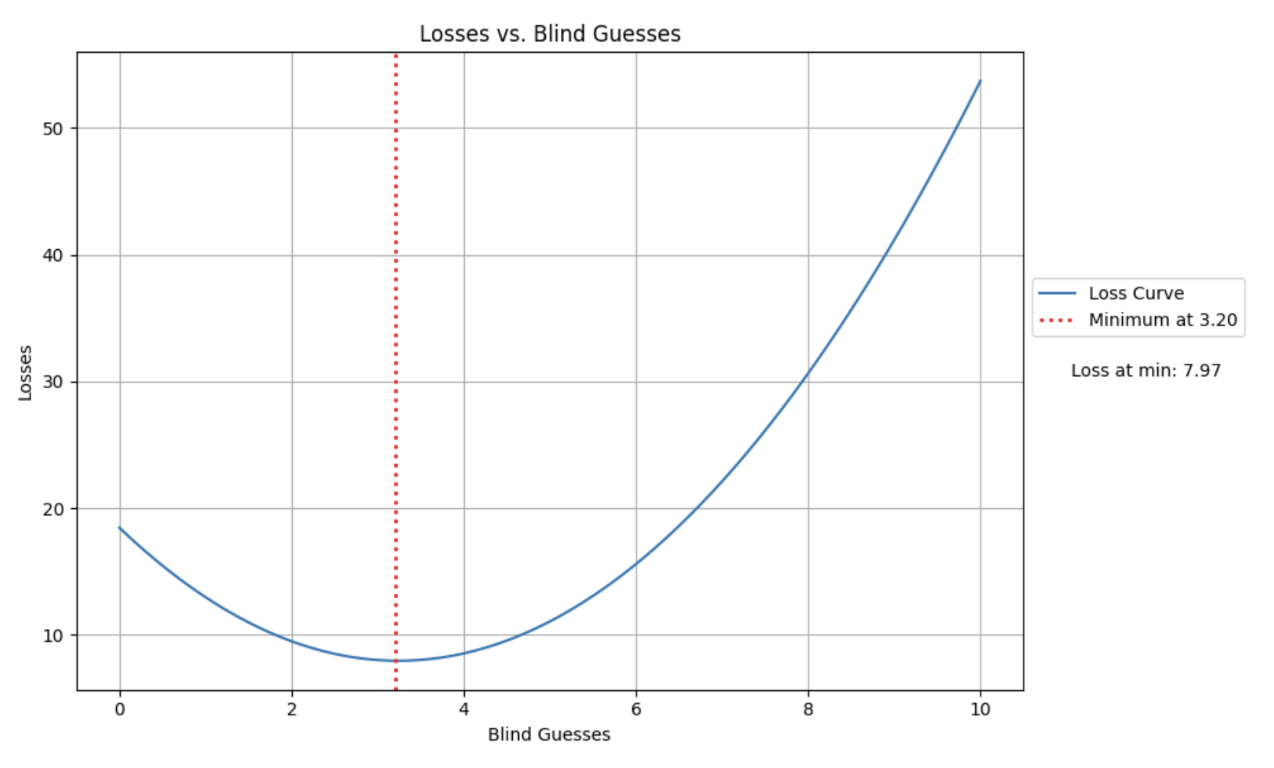
\includegraphics[width=0.6\textwidth]{images/naive_function.png}
    \caption{A graph representation of the loss as the algorithm guessed on the range of [0,10]}
    \label{fig:naive_function}
\end{figure}

After we explored and recorded our results from ChatGPT we transitioned to fine-tuning an existing model
in order to see if performance is noticably better with a model which has been exposed to and trained
on the exact data format we are using. 

\subsection{GNNs}
For the final phase of the avaluation we aim to create an train a GNN from scratch. For the data, we have 
created a script which takes the functions from PrimeVul and converts them into machine readable graphs. 
These graphs represent the information flow of a function and will allow the model to "read" through the code
and see any vulnerabilities or irregularities that could lead to issues such as memory overflow. While we have 
not yet created the GNN, we are optimistic about this approach as it is the one which gets the most exposure
to our data and therefore the most opportunity to properly learn vulnerability identification.

\begin{figure}[htbp]
    \centering
    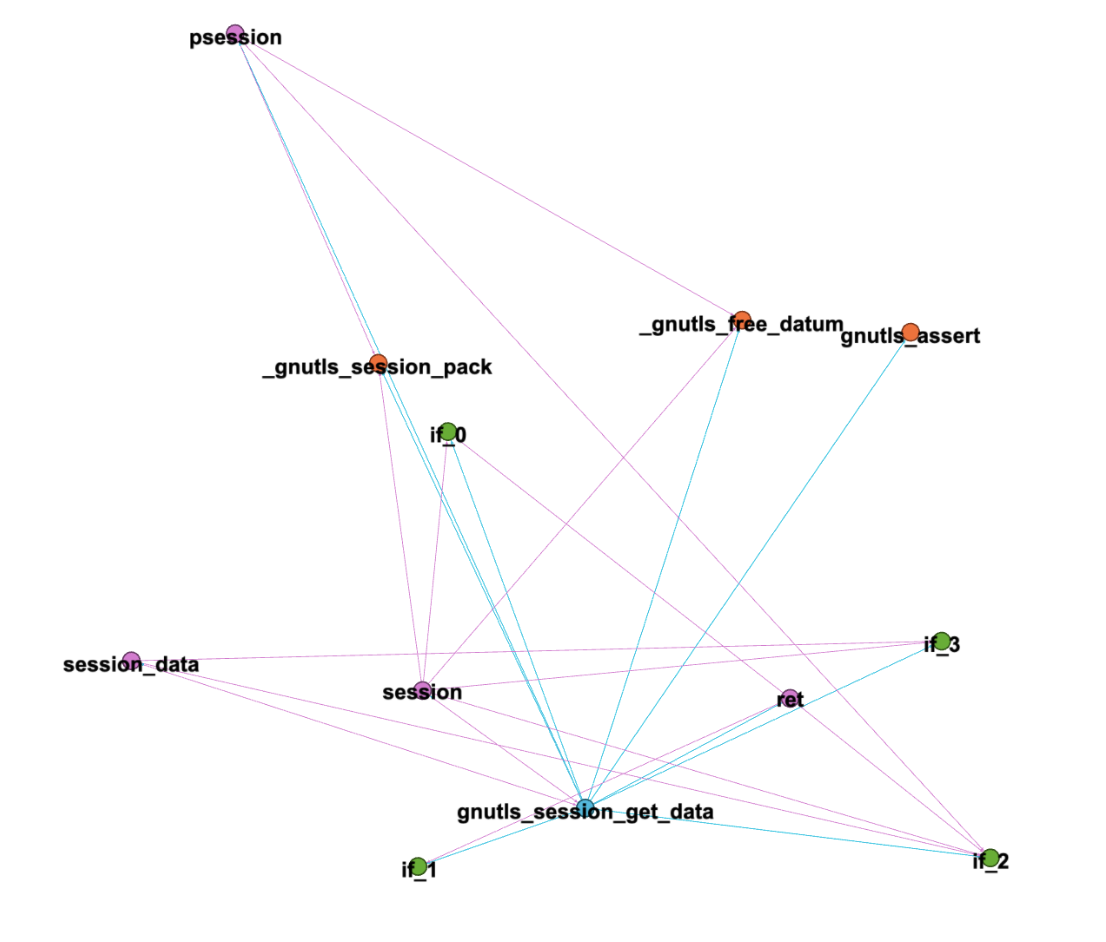
\includegraphics[width=0.5\textwidth]{images/gnn_data.png}
    \caption{A graph representation of an example C function from the dataset}
    \label{fig:gnn_data}
\end{figure}

\section{Transformer Block Overview}

Transformers are neural network architectures designed to process inputs represented as unordered sets of tokens. Each token \( x_n^{(0)} \) is a vector in \( \mathbb{R}^D \), and the full input is arranged as a matrix \( X^{(0)} \in \mathbb{R}^{D \times N} \), where \( N \) is the number of tokens and \( D \) is the feature dimension. This design allows transformers to handle diverse data types, such as text or image patches, using a unified architecture. As Turner notes, this removes the need for ``bespoke handcrafted architectures for mixing data of different modalities' \cite{turner2024introductiontransformers}. The transformer operates by applying a block of operations repeatedly to the input:

\[
X^{(m)} = \text{transformer-block}(X^{(m-1)})
\]

Each block consists of two main stages:
\begin{itemize}
  \item \textbf{Stage 1: Self-Attention across the sequence}
  \item \textbf{Stage 2: Multi-Layer Perceptron (MLP) across features}
\end{itemize}

\subsection{Stage 1: Self-Attention}

Self‐attention allows each token to incorporate information from the entire sequence by computing a weighted sum of all input representations.  Given input matrix \(X^{(m-1)}\in\mathbb{R}^{D\times N}\), we first project into queries and keys:
\[
q_n \;=\; U_q\,x_n,\qquad
k_n \;=\; U_k\,x_n,
\quad
U_q,\,U_k\in\mathbb{R}^{d_k\times D},\;n=1,\dots,N.
\]
Next, we form the raw score matrix \(W\in\mathbb{R}^{N\times N}\) with scaled dot‐products:
\[
W_{n,n'}
=\frac{q_n^{\!\top}k_{n'}}{\sqrt{d_k}}
\qquad
(n,n'=1,\dots,N).
\]
We then normalize each row of \(W\) via a softmax to obtain the attention weights:
\[
A_{n,n'}
=\mathrm{softmax}\bigl(W_{n,\ast}\bigr)_{n'}
=\frac{\exp\bigl(W_{n,n'}\bigr)}
      {\sum_{n''=1}^N\exp\bigl(W_{n,n''}\bigr)}.
\]
Finally, the output of the self‐attention layer is the weighted sum
\[
Y^{(m)}
= X^{(m-1)}\,A^{(m)},
\]
where \(A^{(m)}\) collects the weights \(A_{n,n'}\).  
This introduces the projections 
\[
q_n = U_q x_n,\quad k_n = U_k x_n,
\]
which map each input vector into a “query” and “key” space where similarity scores are computed.  In effect, self-attention re-expresses each vector as a weighted sum of all inputs: if \(A\) and \(B\) are similar (high dot-product in query/key space), then their outputs both become roughly \(A+B\), and similarly for other groups like \(C\) and \(D\).  This lets the model dynamically aggregate information from semantically related tokens.

\subsection{Multi‐Head Self‐Attention (MHSA)}

To allow the model to attend to information in different representational subspaces, multi‐head self‐attention applies \(H\) independent heads in parallel:

\[
\text{head}_h^{(m)}
= V_h \,X^{(m-1)}\,A_h^{(m)},
\qquad h=1,\dots,H,
\]
where each attention matrix is
\[
[A_h^{(m)}]_{n,n'}
=\frac{\exp\bigl((k_{h,n}^{(m)})^\top q_{h,n'}^{(m)}\bigr)}
      {\sum_{n''=1}^N\exp\bigl((k_{h,n''}^{(m)})^\top q_{h,n'}^{(m)}\bigr)},
\]
and
\[
q_{h,n}^{(m)}=U_{q,h}^{(m)}\,x_n^{(m-1)},
\quad
k_{h,n}^{(m)}=U_{k,h}^{(m)}\,x_n^{(m-1)}.
\]

Rather than summing the heads, we **concatenate** their outputs and apply a final linear projection \(W^O\in\mathbb{R}^{D\times (H\,D)}\):

\[
Y^{(m)}
= W^O \;\bigl[\text{head}_1^{(m)} \,\|\, \text{head}_2^{(m)} \,\|\, \cdots \,\|\, \text{head}_H^{(m)}\bigr],
\]
where \(\|\) denotes concatenation along the feature dimension.  


\subsection{Stage 2: MLP Across Features}

After self-attention, each token's vector is refined using a non-linear transformation, applied independently across tokens:

\[
x_n^{(m)} = \text{MLP}(y_n^{(m)})
\]

This operation is akin to the update step in Graph Neural Networks. \cite{turner2024introductiontransformers}

\subsection{Stabilization: Residual Connections and Normalisation}

Each sub-layer is wrapped with a residual connection:

\[
x^{(m)} = x^{(m-1)} + \text{residual}(x^{(m-1)})
\]

and uses \textbf{Layer Normalisation} (referred to in the paper as ``TokenNorm''):

\[
\text{LayerNorm}(x_{d,n}) = \frac{x_{d,n} - \mu_n}{\sqrt{\sigma_n^2}} \gamma_d + \beta_d
\]

where

\[
\mu_n = \frac{1}{D} \sum_{d=1}^D x_{d,n}, \quad \sigma_n^2 = \frac{1}{D} \sum_{d=1}^D (x_{d,n} - \mu_n)^2
\]

and \( \gamma_d, \beta_d \) are learned scale and shift parameters.

\subsection{Positional Encoding}

Because transformers are permutation-invariant, they require additional information to capture token order. This is done by adding or concatenating a positional embedding to each token:

\[
x_n^{(0)} = W p_n + e_n
\]

where \( p_n \) is the input patch or token, \( W \) is the patch embedding matrix, and \( e_n \) is the position embedding. \cite{turner2024introductiontransformers}

\subsection{Conclusion}

The transformer architecture consists of stacked transformer blocks, each combining multi-head self-attention and MLP layers, along with residual connections and layer normalization. By processing sequences in this way, transformers can model complex dependencies across tokens and have become a foundational tool in modern machine learning.

\section{CodeT5}
Following the standard transformer architecture, CodeT5 extends the encoder-decoder model for programming tasks by treating both code and natural language as sequences. It incorporates code-specific pretraining objectives, such as masked span prediction and identifier-aware masking, allowing it to better capture structural and semantic features of code. This enables CodeT5 to excel at code generation, summarization, translation, and understanding tasks across multiple programming languages. 

\subsection{Training Procedure}

Our code fine-tunes the CodeT5-base model by first loading the pre-trained model and tokenizer, which process code as sequences of tokens, enabling the transformer's self-attention mechanisms to model contextual relationships. Then using the pandas library the data is formatted in a data frame and for our combined data set, the batch size, steps per epoch, and epochs are calculated to cover the data set. Entering the training loop, each batch is tokenized, and passed through the model. The model outputs a 2-dimensional vector so that it can perform cross entropy loss in order to fine tune parameters using gradient descent. The script outputs the following features in the log for bookkeeping and for checking that the model is functioning:
\begin{itemize}
\item Batch Size
\item Current Epoch
\item Current Step
\item The loss, accuracy, and the predictions paired with their actual classification
\item The average loss over the epoch
\item Time to complete the epoch
\end{itemize}

\begin{figure}[htbp]
    \centering
    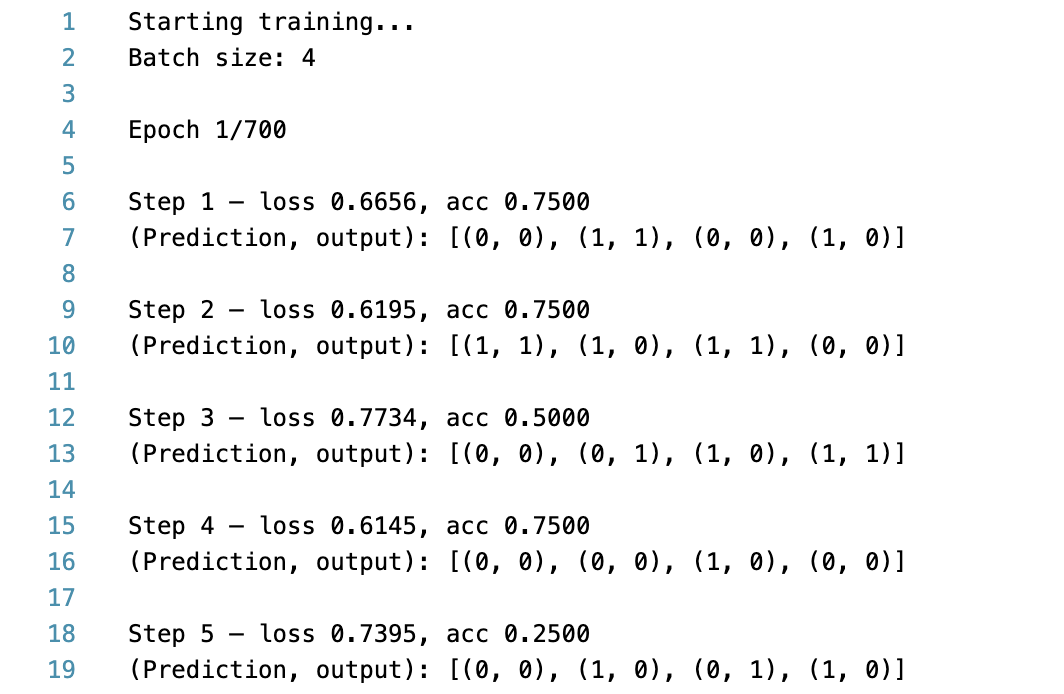
\includegraphics[width=0.5\textwidth]{images/training_log_example.png}
    \caption{Example first few lines from the log file after training}
    \label{fig:training_log_example}
\end{figure}

\begin{figure}[htbp]
    \centering
    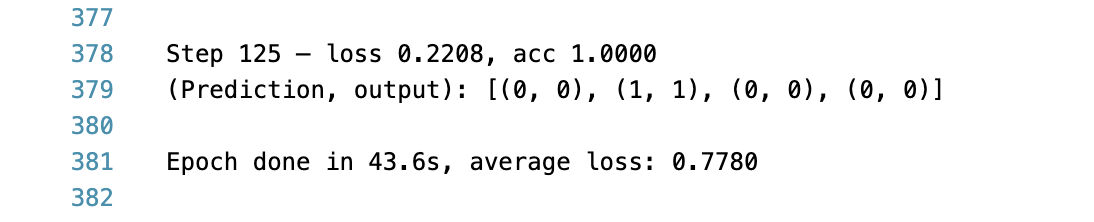
\includegraphics[width=0.5\textwidth]{images/training_log_example2.png}
    \caption{Example of log file at the end of an epoch}
    \label{fig:training_log_example2}
\end{figure}
\bigskip

\pagebreak

The batch size was set as four through trial and error on the Boston College High Performance Computer. Four data points per batch allowed for the GPU to perform the training without exceeding the GPU's memory. The following steps per epoch and epochs were calculated to cover as much of the data as a result of the batch size being restricted to four. Finally, after logging, the model will repeat this loop until all epochs are completed and then save out the model to a folder.

\subsection{Testing The Trained Model}

After the training script saves out the model, it is loaded into the test script. This script loads the data in a similar process as the training script. Then, each batch is feed through the model. The data point's true values are appended to an array with their corresponding predictions being appended to a separate array. These arrays are compared to ensure that the model has been feed all the entries. Then, using the sklearn library, the following metrics are calculated and outputted to a log file:

\begin{itemize}
\item Accuracy Score
\item Precision Score
\item Recall Score
\item F1 Score
\end{itemize}

\section{Model Evaluation}

The model was trained on two data sets -- the combined data set and the Prime-Vul data set. Table~\ref{tab:metrics} summarizes the overall classification metrics for each model.

\begin{table}[ht]
  \centering
  \begin{tabular}{|l|c|c|}
    \hline
    \textbf{Metric}   & \textbf{Combined Data Set Model} & \textbf{Prime-Vul Data Set Model} \\ 
    \hline 
    Accuracy          & 88.48\%                          & 77.74\%                  \\ 
    \hline
    Precision         & 32.96\%                          & 32.16\%                  \\ 
    \hline
    Recall            & 95.49\%                          & 76.11\%                  \\ 
    \hline
    F1 Score          & 49.01\%                          & 45.21\%                  \\ 
    \hline
  \end{tabular}
  \caption{Overall performance metrics on the two evaluation datasets.}
  \label{tab:metrics}
\end{table}

The Combined Data Set model achieves a high accuracy of 88.48 \%, driven largely by its ability to correctly identify the majority class (non-vulnerable functions). Its recall of 95.49 \% indicates that it successfully captures almost all true vulnerable cases; however, at the expense of precision (32.96 \%), leading to a moderate F1 Score of 49.01 \%.  

In contrast, the Prime-Vul Data Set model shows lower overall accuracy (77.74 \%) and recall (76.11 \%), reflecting the increased difficulty of this focused subset. Its precision remains similar (32.16 \%), yielding an F1 Score of 45.21 \%. This suggests that while the model generalizes well across the full dataset, its performance degrades somewhat when restricted to the prime-vulnerability domain.

To better understand where each model makes errors, we examine the confusion matrices below. Table~\ref{tab:confmat-large} shows the Combined Data Set results on 27,900 examples, and Table~\ref{tab:confmat-small} shows the Prime-Vul Data Set results on 7,456 examples.

\begin{table}[ht]
  \centering
  \begin{tabular}{c|cc}
    & \textbf{Pred = 0} & \textbf{Pred = 1} \\ \hline
  \textbf{Actual = 0} & 23,141 & 3,141 \\
  \textbf{Actual = 1} &    74  & 1,544 \\
  \end{tabular}
  \caption{Confusion matrix for the Combined Data Set model (27,900 examples).}
  \label{tab:confmat-large}
\end{table}

\pagebreak

In the Combined Data Set confusion matrix, the model correctly labels 23,141 of 26,282 non-vulnerable samples (true negatives) and 1,544 of 1,618 vulnerable samples (true positives). Only 74 vulnerable samples are missed (false negatives), confirming the high recall. However, 3,141 non-vulnerable samples are incorrectly flagged as vulnerable (false positives), which drives down the precision.

\begin{table}[ht]
  \centering
  \begin{tabular}{c|cc}
    & \textbf{Pred = 0} & \textbf{Pred = 1} \\ \hline
  \textbf{Actual = 0} & 5,112 & 1,444 \\
  \textbf{Actual = 1} &  215  &   685 \\
  \end{tabular}
  \caption{Confusion matrix for the Prime-Vul Data Set model (7,456 examples).}
  \label{tab:confmat-small}
\end{table}

On the Prime-Vul Data Set, the model still identifies the majority of non-vulnerable samples correctly (5,112 true negatives), but it misses more vulnerable cases (215 false negatives) relative to the smaller positive class (900 samples). The increase in both false positives (1,444) and false negatives reflects the greater challenge of this domain and explains the drop in both accuracy and recall.

Overall, these results highlight the trade-off between capturing as many true vulnerabilities as possible (recall) and avoiding excessive false alarms (precision). Tuning this balance will depend on the practical needs of the security pipeline: whether catching every possible vulnerability is paramount or reducing investigator workload from false positives is more critical.


\subsection{Next Steps for Project}
The following is a general list of the steps we plan to take through the rest of the semester.
This is a rough outline as we don't yet know what the exact steps are going to entail and is subject to change as we progress through the project.

\begin{enumerate}
    \item Finalize and expand the graph database to contain the entire train, test and validation function
      
      (Estimated : 2 hours)
    \item Starting from scratch, implement the research done by Alex and Bryan to create a GNN from scratch using the formatted graph data as training input.

      (Estimated : 70 hours)

    \item Evaluate the from scratch model against the previously explored options to understand the impact
      of architectural decisions in the models creation

      (Estimated : 5 hours)
\end{enumerate}

\subsection{Contribution Timeline}
\textbf{01/22: Alex, Sara, Drew, Bryan} First team meeting where project ideas were
brainstormed. Google doc was created to store ideas and research \\
\textbf{01/23: Drew, Bryan} Team meeting with Prof. Bento to discuss project ideas.
Code Vulnerability project was chosen \\
\textbf{01/27: Alex, Sara, Drew, Bryan} Team meeting to discuss strategy, proficiencies, 
and research approach \\
\textbf{01/29: Alex} Research on VulKG knowledge-graph. Wrote the abstract. \\
\textbf{01/30: Drew} Research on DiverseVul database. Wrote behaviours section \\
\textbf{01/30: Sara} Research to find papers and literature related to the topic \\
\textbf{01/31: Alex, Drew} Meeting with Professor Bento, discussing progress and databases \\
\textbf{01/31: Sara} Research to find so Python databases \\
\textbf{01/31: Alex} Research on the PrimeVul database and wrote about it. \\
\textbf{02/01: Bryan} Research on current machine learning cybersecurity issues. Wrote
introduction. Found and wrote up a summary about the OSV database \\
\textbf{02/01: Drew} Wrote the Related Works section \\
\textbf{02/02: Drew} Created code to run the functions on ChatGPT and record the loss \\
\textbf{02/03: Alex} Created code to graph data from ChatGPT vulnerability detection loss \\
\textbf{02/05: Alex} Tested "blind guesses" data on first 1000 entries in train dataset \\
\textbf{02/07: Alex, Drew, Bryan, Sara} Researched the NVD API, and tried to get it to run faster \\
\textbf{02/08: Drew} Researched fine-tuning of existing models for improved accuracy \\
\textbf{02/15: Alex} Researched Vul-LMGNN, a pre-existing model using GNN architecture \\
\textbf{02/16: Alex} Researched pre-existing models, including CodeT5 and CodeBERT for fine-tuning \\
\textbf{02/16: Bryan} Experimented with batch and parallelizing the API script \\
\textbf{02/17: Alex} Attempted to fine-tune CodeBERT on first 1000 entries of dataset \\
\textbf{02/18: Drew} Decreased the load time of CVSS scores from hours to minutes through a web scraping algorithm instead of an API call \\
\textbf{02/25: Alex, Drew, Bryan, Sara} Scraped 44,000 entries each in the train dataset to get their CVSS 2.0 vulnerability score and put into reformatted dataset \\
\textbf{02/26: Alex} Scraped for validation dataset \\
\textbf{02/26: Bryan} Began implementing codeT5 and troubleshooting \\
\textbf{03/08: Drew} Created an algorithm to format data for mistral fine-tuning \\
\textbf{03/09: Drew} Ran fine tuning on Mistral through a python script (failure) \\
\textbf{03/10: Alex} Scraped for test dataset \\
\textbf{03/13: Alex, Drew, Bryan, Sara} Met to discuss architecture, discovered GNNs \\
\textbf{03/17: Alex, Drew} Researched CPGs \\
\textbf{03/18: Alex} Read paper on ANGEL model \\
\textbf{03/19: Drew} Created an algorithm to create graphs from code snippets and functions \\
\textbf{03/19: Bryan} Read and wrote about the general transformer architecture \\
\textbf{03/19: Sara} Research on cost of data breach in the past years and how these have been handled \\
\textbf{03/19: Drew} Research on GNNs \\
\textbf{03/20: Sara} Read other articles about problems of ML in the computer security field \\
\textbf{03/20: Alex} Updated datasets in github to contain "func\_hash", file\_info.json, and file\_contents zip \\
\textbf{03/20: Alex} Wrote up sections on Flawfinder, ANGEL \\
\textbf{03/20: Alex} Researched AMPLE GNN model \\
\textbf{03/20: Bryan} Further implementing codeT5 and test train speeds and losses \\
\textbf{03/20: Drew} Wrote the experimentation section of the LaTeX \\
\textbf{03/21: Sara} Researched more about the mechanisms behind the pitfalls \\
\textbf{03/21: Sara} Analyzed how much the databases have been used by the research community (paperswithcode website) \\
\textbf{03/21: Alex} Wrote about AMPLE model \\
      

% Bibliography
\bibliographystyle{ieeetr}  % Changed to IEEE style for numbered references
\bibliography{bibliography}  % This refers to bibliography.bib

\end{document}
